%%%%%%%%%%%%%%%%%%%%%%%%%%%%%%%%%%%%%%%%%%%%%%%%%%%%%%%%
%%%%%%%%%-----RMIT SPACE POSTER ------------%%%%%%%%%%%%
%%%%%%%%%%%%%%%%%%%%%%%%%%%%%%%%%%%%%%%%%%%%%%%%%%%%%%%%
%%%%%%%%%%%%%%%%%%%%%%%%%%%%%%%%%%%%%%%%%%%%%%%%%%%%%%%%
% a0poster Portrait Poster
%
% The a0poster class was created by:
% Gerlinde Kettl and Matthias Weiser (tex@kettl.de)
% This a0poster class was adapted by:
% Ava Francesca Battocchio (battocch@msu.edu)
% 
% License:
% CC BY-NC-SA 3.0 (http://creativecommons.org/licenses/by-nc-sa/3.0/)
%
% Author/Designer: Timothy Kodikara
%
%% Note: CRC and SERC logos are included in the /figures folder if you might want to use them.
%%%%%%%%%%%%%%%%%%%%%%%%%%%%%%%%%%%%%%%%%
%----------------------------------------------------------------------------------------
%	PACKAGES AND OTHER DOCUMENT CONFIGURATIONS
%----------------------------------------------------------------------------------------
\documentclass[a0,portrait]{a0poster}
%%
\usepackage[top=5cm, bottom=0.3cm, left=5cm, right=3cm]{geometry}
\usepackage[compact]{titlesec}
\usepackage{multicol} % This is so we can have multiple columns of text side-by-side
\columnsep=100pt % This is the amount of white space between the columns in the poster
\columnseprule=15pt % This is the thickness of the blue line between the columns in the poster
\usepackage[svgnames]{xcolor} % Specify colors by their 'svgnames', for a full list of all colors available see here: http://www.latextemplates.com/svgnames-colors
%\usepackage{times} % Use the times font
\usepackage{palatino} % Uncomment to use the Palatino font
\usepackage{xkeyval}
\usepackage{graphicx} % Required for including images
\setlength{\abovecaptionskip}{5pt plus 5pt minus 3pt}
\graphicspath{{figures/}} % Location of the graphics files
\usepackage{booktabs} % Top and bottom rules for table
\usepackage[font=small,labelfont=bf]{caption} % Required for specifying captions to tables and figures
\usepackage{amsfonts, amsmath, amsthm, amssymb} % For math fonts, symbols and environments
\usepackage{csquotes}
\usepackage{wrapfig} % Allows wrapping text around tables and figures
%\usepackage[pdftex]{color}
\def\columnseprulecolor{\color{Maroon}}%
\usepackage{framed}
\colorlet{frameborder}{Maroon}
\documentclass{article}


\usepackage[style=numeric]{biblatex}
\bibliography{JPBM-Brand_Auth.bib}
\usepackage{cite}
\AtBeginBibliography{\tiny}

%----------------------------------------------------------------------------------------
%	POSTER HEADER 
%----------------------------------------------------------------------------------------
% The header is divided into three boxes:
% The widths of these boxes can be easily edited to accommodate your content as you see fit
\begin{document}
%\hspace*{0.2cm}
\begin{minipage}[c]{\linewidth}
\vspace{0.1cm}
\noindent\makebox[\textwidth][c]{
\begin{minipage}[c]{0.10\linewidth}
\vspace{0pt}\raggedright
\hspace{1cm}

\includegraphics[scale=4,width=\linewidth]{LUC_stacked.png}
\end{minipage}
\hfill
\begin{minipage}[c]{0.70\textwidth}
\centering
\Huge \color{Maroon} \textbf{Effects of Transparent Brand Communication on Perceived Brand Authenticity and Consumer Responses}\\[0.5cm]
\large \color{Black} \textbf{Jing Yang, Ph.D.^{1}$ and Ava Francesca Battocchio, M.S. $^{2} $}\\[0.2cm] % Author(s)
\small 1. School of Communication, Loyola University Chicago \\[0.1cm] % University
\small 2. Department of Advertising and Public Relations, Michigan State University\\[0.1cm] % Affiliation 2
\small \texttt{Correspondence: jyang13@luc.edu}\\
\end{minipage}
%\hfill
\begin{minipage}[c]{0.15\textwidth}
\vspace{0pt}\raggedleft

\includegraphics[scale=3,width=\linewidth]{MSU_Wordmark.png}
\hspace{1cm}
\end{minipage}}
\\[0.1cm]%
% A bit of extra whitespace between the header and poster content
%----------------------------------------------------------------------------------------
\color{Maroon}\setlength\FrameRule{25pt}
\begin{framed}
\vspace{0.5cm}
\begin{multicols}{2} % This is how many columns your poster will be broken into, a portrait poster is generally split into 2 columns
%----------------------------------------------------------------------------------------
%	INTRODUCTION
%----------------------------------------------------------------------------------------
\color{Maroon}
\section*{Abstract}
\color{Black}
This study explores the influence of transparent brand communication on consumers' perception of brand authenticity, and its further impact on consumers' attitude, trust, and behavioral intention towards the brand. Through a 2x2 online experiment design, this study examined the variation in consumers' perception and responses, while connecting the literature of brand transparency and authenticity. Individuals' difference in moral identity centrality was examined as a moderator in the study
\color{Maroon}
\section*{Literature Review}
\color{Black}
  \color{Maroon} \textbf{\emph{Brand Transparency:}} \color{Black}
Transparency utilizes openness\autocite{parris_exploring_2016} and brand accountability\autocite{yoo_brand_2014} to communicate information gathering,funding, sharing, access,and disclosure \autocite{phillips_online_2009}\autocite{wojdynski_measuring_2018} \autocite{yoo_brand_2014}\autocite{brandao_impact_2018}.Prior studies reveal consumer perceptions of brand transparency results in trust-building, positive attitudes, and behavioral intentions \autocite{reynolds_moral_2008}.\\
\\
  \color{Maroon} \textbf{\emph{Brand Authenticity:}} \color{Black} Authenticity contributes principal positive value to a brand's image \autocite{keller_strategic_1998}\autocite{ballantyne_evolution_2006} and identity \autocite{beverland_crafting_2005}\autocite{kapferer_new_2008}. Authentic brands are distinguished through their sincerity, stability, endurance, consistency, credibility, originality, truthfulness, genuineness, realness, and dissociation from commercial motives \autocite{bruhn_brand_2012}\autocite{grayson_consumer_2004}\autocite{ballantyne_evolution_2006}\autocite{beverland_real_2006}\autocite{holt_why_2002}. 
  \\
  
\\ 
\\
    \color{Maroon} \textbf{\emph{Moral Identity:}} \color{Black}Individuals’ moral identity (MI) centrality refers to “the degree to which being moral is a central or defining characteristic of a person’s sense of self” \autocite{blasi_moral_1994}.
    Aquino and his colleagues \autocite{aquino_self-importance_2002}\autocite{aquino_testing_2009}, operationalized MI centrality as a set of moral traits that are stable to one’s self-conception and guides behavior. 
    \\
   \begin{center}
  \color{Maroon} \textbf{RQ:} \color{Black}  Which kind of transparent brand communication (production transparency vs. cost transparency vs. both) will be perceived with higher brand transparency? \\

  \end{center}
  
  \begin{wrapfigure}{R}{0.30\textwidth}
\centering
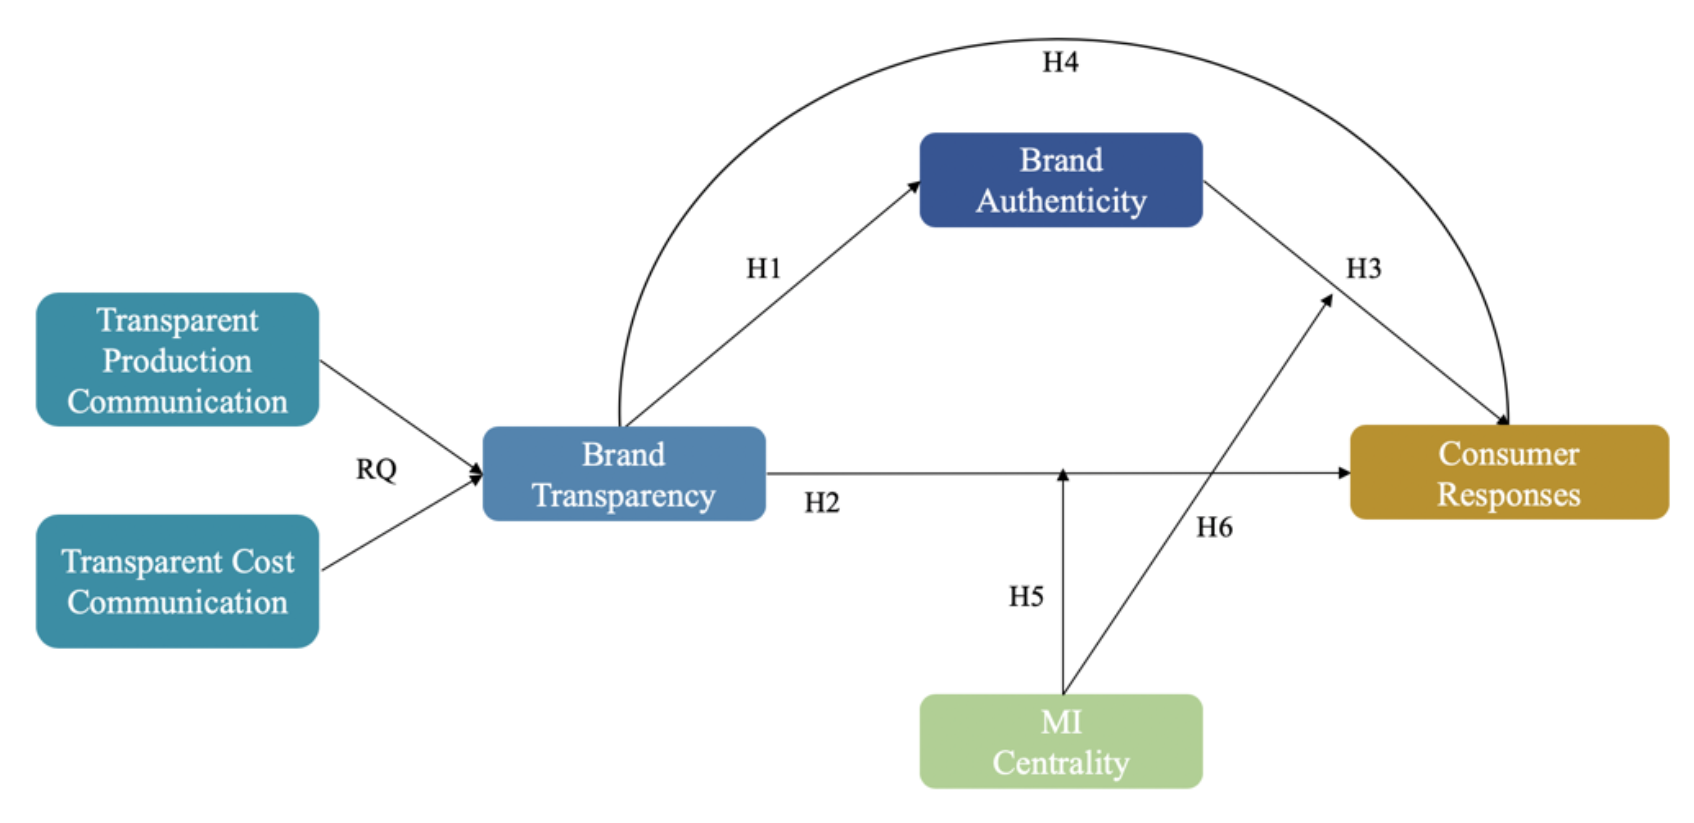
\includegraphics[scale=1.3]{figures/Figure1}
\captionof{figure}{\color{DarkSlateGrey} Hypothesis Model}
\label{ALICerros}
\end{wrapfigure}
\\
\color{Maroon}
\textbf \\{H1:} \color{Black}Brand transparency will positively contribute to consumers' perception of the brand's authenticity. \\

\color{Maroon}
\textbf{H2:} \color{Black} Brand transparency will positively relate to consumers’ a) trust, b) attitude and c) behavioral intentions towards the brand.\\
\\
\color{Maroon}
\textbf{H3:} \color{Black} Brand authenticity will positively relate to consumers’ a) trust, b) attitude and c) behavioral intentions towards the brand.\\
\\
\color{Maroon}
\textbf{H4:} \color{Black} Brand authenticity will mediate the positive relationship between brand transparency and consumers’ a) trust, b) attitude, and c) behavioral intentions towards the brand.\\
\\
\color{Maroon}
\textbf{H5:} \color{Black}  Individuals’ MI centrality would moderate the impact of brand transparency on consumers’ a) trust, b) attitude, and c) behavioral intentions towards the brand, such that people with higher moral identity centrality are more likely to respond positively towards brand with higher brand transparency.\\
\\
\color{Maroon}
\textbf{H6:} \color{Black} Individuals’ MI centrality would moderate the impact of brand authenticity on consumers’ a) trust, b) attitude, and c) behavioral intentions towards the brand,
such that people with higher moral identity centrality are more likely to respond positively towards brands with higher brand authenticity.
}
%----------------------------------------------------------------------------------------
%	METHODS
%---------------------------------------------------------------------------------------- 
\color{Maroon}
\section*{Methods}
\color{Black}
 This study utilized an online between-subject, 2x2 experiment design	
\begin{itemize}
    \item Cost Transparency (Present or not) x Production Transparency (Present or not) 
\end{itemize}
\\
\color{Maroon}
\textbf{\emph{Stimuli Development}}
\color{Black}
\begin{itemize}
    \item Created fictitious apparel brand called \textit{A\text{\_} Tee} with mock-up of e-commerce website
    \item Participants were assigned to review one of four conditions:
    \end{itemize}
   
   
   %\begin{wrapfigure}{R}{0.25\textwidth}
\begin{center}
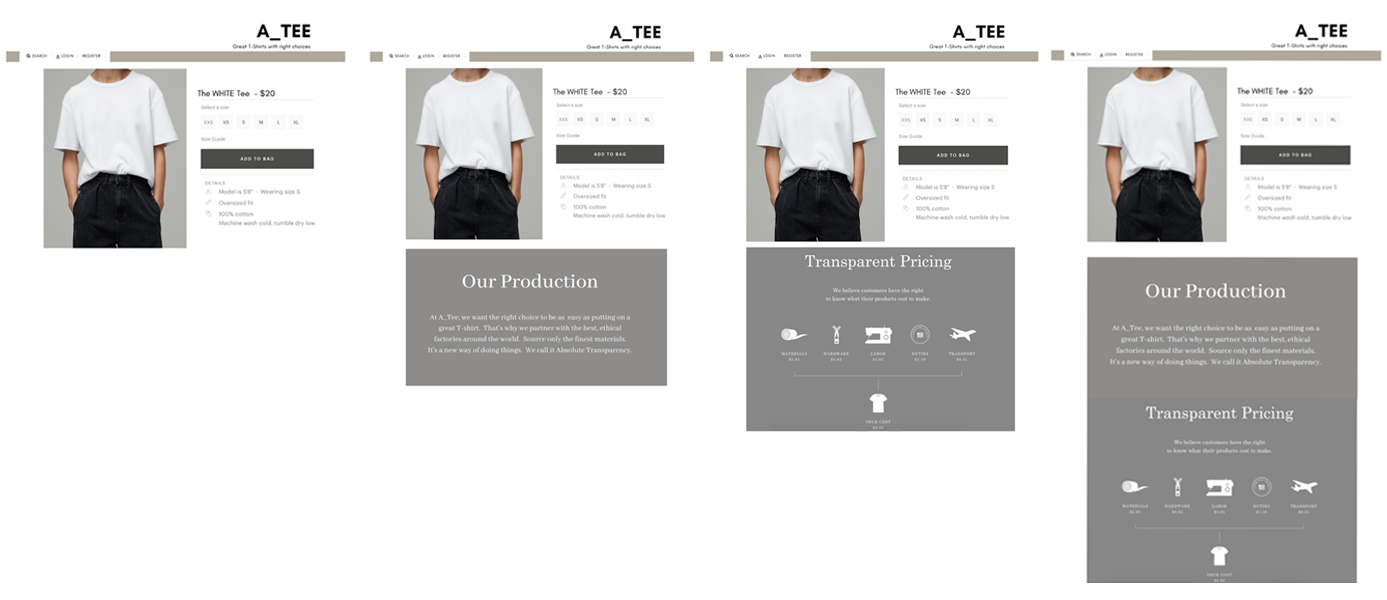
\includegraphics[width=1.0\linewidth]{AEJMC-Brand_Auth-Stimuli-Figure}
\captionof{figure}{\color{DarkSlateGray}(far left)\textbf{\emph{ Control:}} unisex tee photo plus price, material and size options \\ (left)\textbf{\emph{ Transparent Production:}} Control descriptors plus partnered factories and material sourcing (right)\textbf{\emph{ Transparent Price:}} Control descriptors plus costs of material, hardware, labor, duties, and transportation fees \\ (far right) \textbf{\emph{Transparent Price and Production:}} Control descriptors plus both price and production descriptors}
\label{ALICerros}
\end{center}

\color{Maroon}
\textbf{\emph{Participants}}
\color{Black}
\begin{itemize}
\item \textit{n=172}
\item Recruited on Amazon Mturk
\begin{itemize}
    \item US participants 
    \item 61.5\text{\%} Male
    \item 79.3\text{\%} White
    \item 51.7\text{\%} Bachelor's Degree
    \item Ages ranged from 21 to 75 (M=39.5, SD=12.235)
    \begin{itemize}
        \item 43.7\text{\%} Millennials (Between 13 to 34)
    \end{itemize}
    \item 71.3\text{\%} Employed full-time
    \item 58.6\text{\%} Annual household income under \text{\$}50,000
\end{itemize}
\color{Maroon}
\textbf{\emph{Measures}}
\color{Black}


\begin{itemize} \item 
\textbf{\emph{Brand Transparency:}} 7-point Likert scale adapted from Kang and Hustvedt (2013).
\end{itemize}
\begin{itemize}
    \item \textbf{\emph{Brand Authenticity:}} 7-point Likert scale adapted from Bruhn et al.(2012).
\end{itemize}
\begin{itemize} \item
\textbf{\emph{Moral Identity (MI) Centrality:}} 7-point Likert scale adapted from Aquino and Reed(2002).
\end{itemize}
\begin{itemize} \item
\textbf{\emph{Brand Trust:}} 7-point Likert scale adapted from
Erdem and Swait (2004).
\end{itemize}
\begin{itemize} \item
\textbf{\emph{Attitude Towards Brand:}} 7-point Likert scale adapted from adapted from Sengupta and Johar (2002)
\end{itemize}
\begin{itemize} \item
\textbf{\emph{Behavioral Intention:}} 7-point Likert scale adapted from Oh et al. (2019)
\end{itemize}
\end{itemize}
%----------------------------------------------------------------------------------------
%	RESULTS
%---------------------------------------------------------------------------------------- 

\color{Maroon}
\section*{Results}
\color{Black}

\begin{center}
\includegraphics[width=0.5\linewidth]{figures/AEJMC-Brand_Auth-Results-Figure 2A }
\captionof{figure}{\color{DarkSlateGrey} Mediation analyses by DV: Trust} 
\label{ALICerros}
\end{center}

\begin{center}
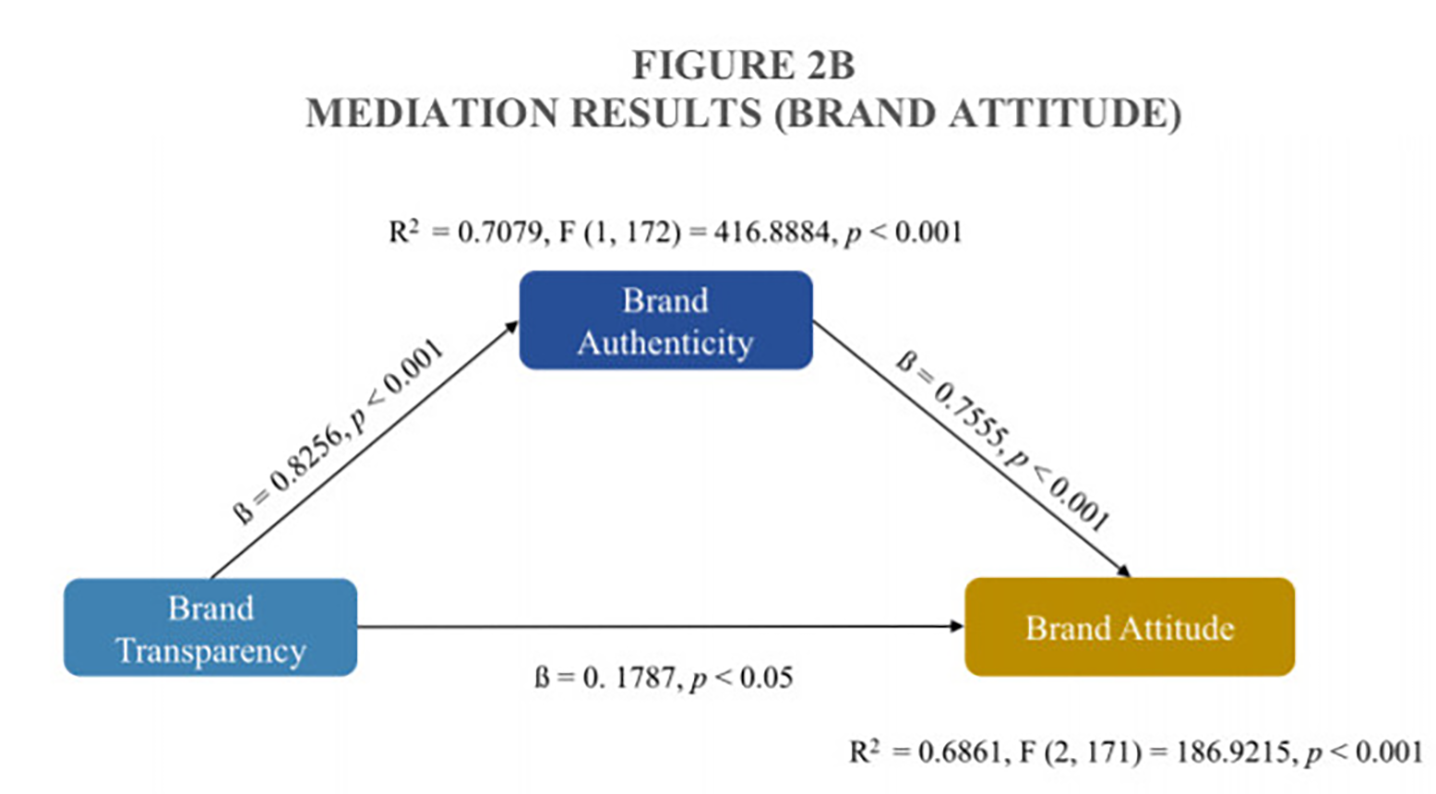
\includegraphics[width=0.5\linewidth]{figures/AEJMC-Brand_Auth-Results-Figure 2B}
\captionof{figure}{\color{DarkSlateGrey} Mediation analyses by DV: Attitude} 
\label{ALICerros}
\end{center}

\begin{center}
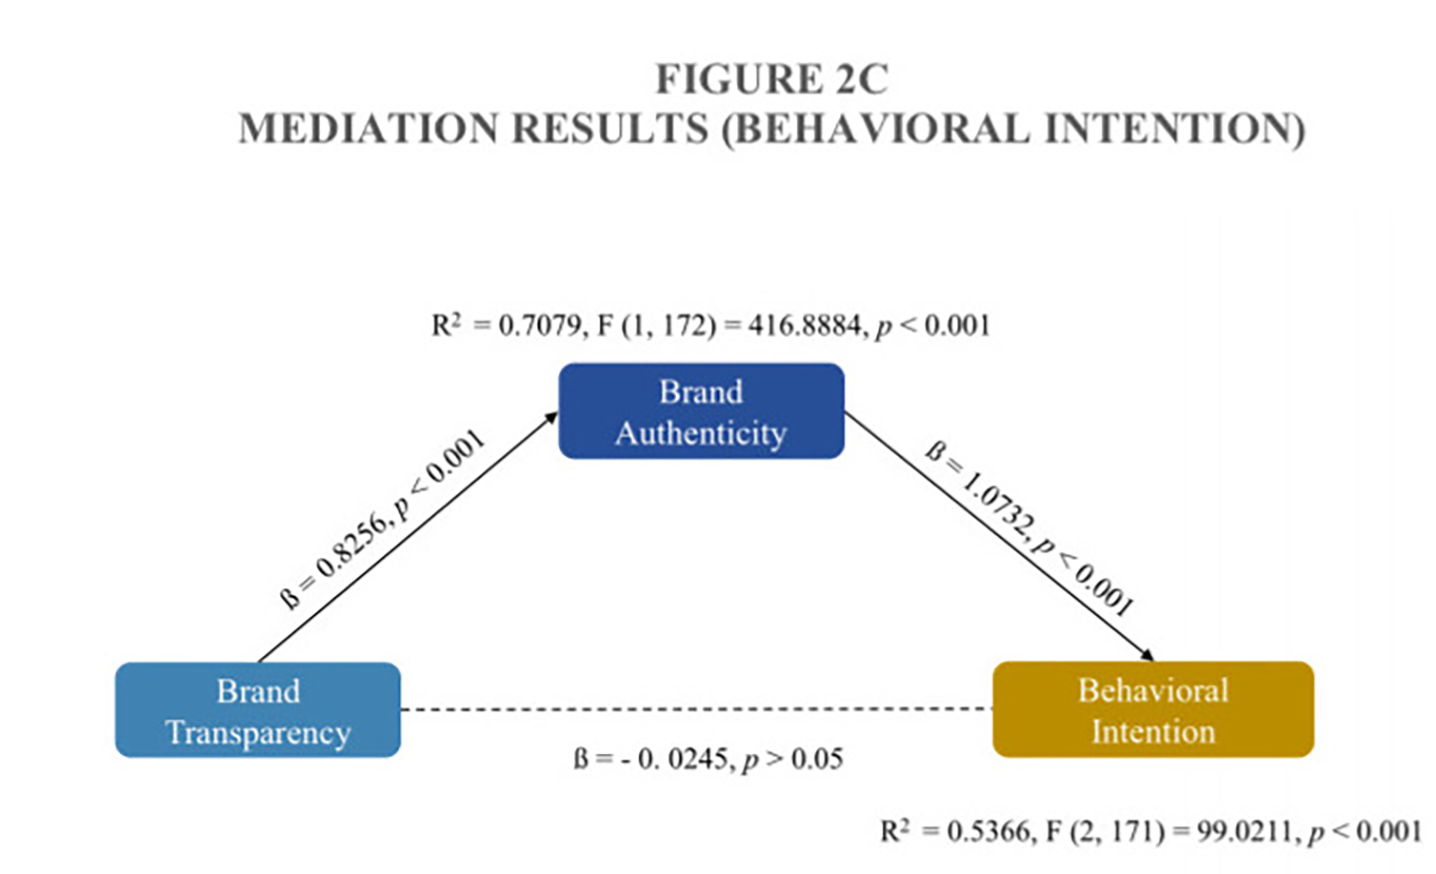
\includegraphics[width=0.5\linewidth]{figures/AEJMC-Brand_Auth-Results-Figure 2C}
\captionof{figure}{\color{DarkSlateGrey} Mediation analyses by DV: Behavior} 
\label{ALICerros}
\end{center}

\begin{center}
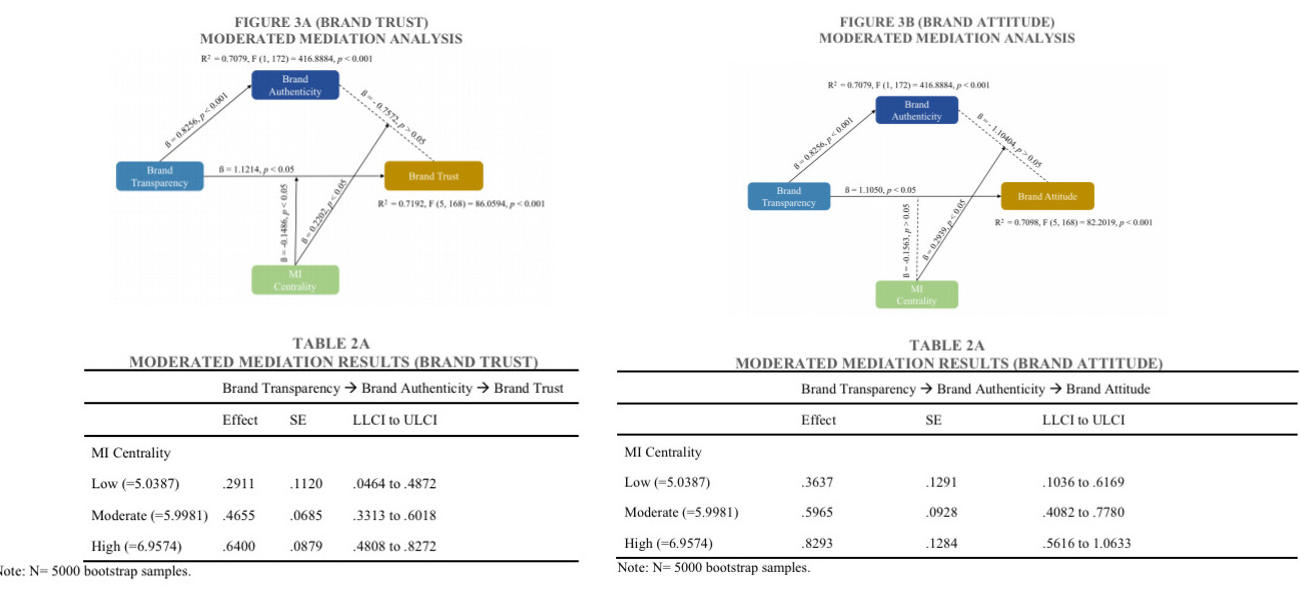
\includegraphics[width=0.7\linewidth]{AEJMC-Brand_Auth-Results-3A_3B}
\captionof{figure}{\color{DarkSlateGrey} Moderated meditation analyses by DV: (left) trust and (right) attitude }
\label{ALICerros}
\end{center}
-----------------------------
%	CONCLUSIONS
%----------------------------------------------------------------------------------------
\color{Maroon}
\section*{Discussion}
\color{Black}
Our findings demonstrated that by revealing the production process and product cost, consumers would view a brand as more authentic and trustworthy. In turn, their positive attitude and purchase intention toward the brand would be more significant. These findings support previous literature that suggests the positive impact of transparent brand communication and brand authenticity on consumer responses. This study also found that individuals’ moral identity (MI) centrality significantly
moderated the relationship between brand transparency and consumers’ responses towards the brand (i.e., trust and attitude), through the mediation of perceived brand authenticity.


%----------------------------------------------------------------------------------------
%	REFERENCES
%----------------------------------------------------------------------------------------
\color{Maroon} \\
\color{Black}
\printbibliography
\end{multicols}
%\textcolor{NavyBlue}{\rule{\linewidth}{15pt}}
\vspace{0.5cm}
\end{framed}
\end{minipage}
%\hspace*{0.1cm}
\end{document}
%----------------------------------------------------------------------------------------
%%%%%%%%%%%%%%%%%%%%%%%%%%%%%%%%%%%%%%%%%%%%%%%%%%